\hypertarget{DelegateTest2_8cc}{
\section{/data/callbackext/Tests/Delegate\-Test2.cc File Reference}
\label{DelegateTest2_8cc}\index{/data/callbackext/Tests/DelegateTest2.cc@{/data/callbackext/Tests/DelegateTest2.cc}}
}
{\tt \#include $<$iostream$>$}\par
{\tt \#include \char`\"{}../Container/Delegate\-List.hpp\char`\"{}}\par
{\tt \#include \char`\"{}../Delegate\-N/Delegate\-N.hpp\char`\"{}}\par
{\tt \#include \char`\"{}../Functor\-N/Functor\-N.hpp\char`\"{}}\par


Include dependency graph for Delegate\-Test2.cc:\begin{figure}[H]
\begin{center}
\leavevmode
\includegraphics[width=208pt]{DelegateTest2_8cc__incl}
\end{center}
\end{figure}
\subsection*{Functions}
\begin{CompactItemize}
\item 
void \hyperlink{DelegateTest2_8cc_a0}{test0} ()
\item 
void \hyperlink{DelegateTest2_8cc_a1}{test1} (int i1)
\item 
void \hyperlink{DelegateTest2_8cc_a2}{test2} (int i1, int i2)
\item 
void \hyperlink{DelegateTest2_8cc_a3}{test3} (int i1, int i2, int i3)
\item 
void \hyperlink{DelegateTest2_8cc_a4}{test4} (int i1, int i2, int i3, int i4)
\item 
void \hyperlink{DelegateTest2_8cc_a5}{test5} (int i1, int i2, int i3, int i4, int i5)
\item 
void \hyperlink{DelegateTest2_8cc_a6}{test6} (int i1, int i2, int i3, int i4, int i5, int i6)
\item 
void \hyperlink{DelegateTest2_8cc_a7}{test7} (int i1, int i2, int i3, int i4, int i5, int i6, int i7)
\item 
void \hyperlink{DelegateTest2_8cc_a8}{test8} (int i1, int i2, int i3, int i4, int i5, int i6, int i7, int i8)
\item 
void \hyperlink{DelegateTest2_8cc_a9}{test9} (int i1, int i2, int i3, int i4, int i5, int i6, int i7, int i8, int i9)
\item 
void \hyperlink{DelegateTest2_8cc_a10}{test10} (int i1, int i2, int i3, int i4, int i5, int i6, int i7, int i8, int i9, int i10)
\item 
int \hyperlink{DelegateTest2_8cc_a11}{main} ()
\end{CompactItemize}


\subsection{Function Documentation}
\hypertarget{DelegateTest2_8cc_a11}{
\index{DelegateTest2.cc@{Delegate\-Test2.cc}!main@{main}}
\index{main@{main}!DelegateTest2.cc@{Delegate\-Test2.cc}}
\subsubsection[main]{\setlength{\rightskip}{0pt plus 5cm}int main ()}}
\label{DelegateTest2_8cc_a11}




Definition at line 77 of file Delegate\-Test2.cc.

References DL::Delegate\-List::add(), DL::create\_\-delegate(), test0(), test1(), test10(), test2(), test3(), test4(), test5(), test6(), test7(), test8(), and test9().

Here is the call graph for this function:\begin{figure}[H]
\begin{center}
\leavevmode
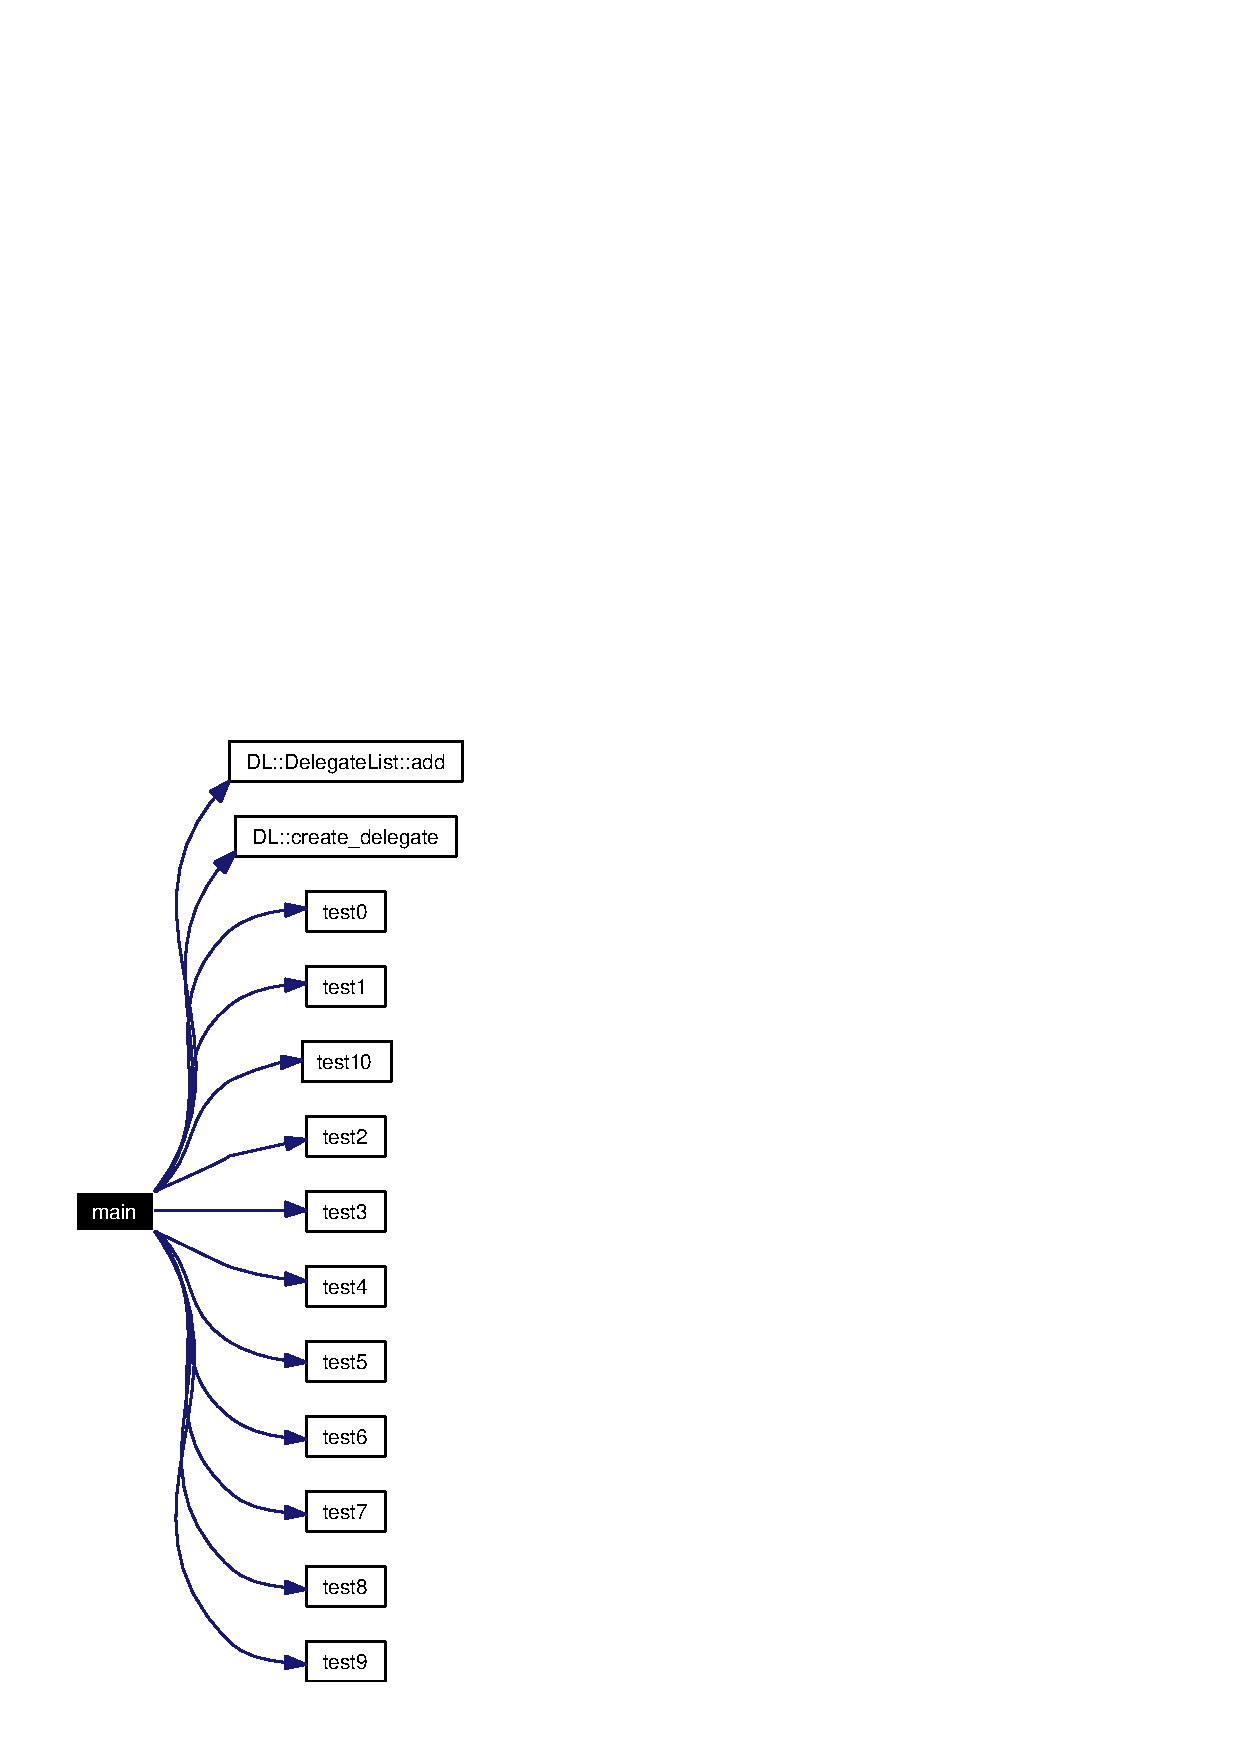
\includegraphics[width=111pt]{DelegateTest2_8cc_a11_cgraph}
\end{center}
\end{figure}
\hypertarget{DelegateTest2_8cc_a0}{
\index{DelegateTest2.cc@{Delegate\-Test2.cc}!test0@{test0}}
\index{test0@{test0}!DelegateTest2.cc@{Delegate\-Test2.cc}}
\subsubsection[test0]{\setlength{\rightskip}{0pt plus 5cm}void test0 ()}}
\label{DelegateTest2_8cc_a0}




Definition at line 27 of file Delegate\-Test2.cc.

Referenced by main().\hypertarget{DelegateTest2_8cc_a1}{
\index{DelegateTest2.cc@{Delegate\-Test2.cc}!test1@{test1}}
\index{test1@{test1}!DelegateTest2.cc@{Delegate\-Test2.cc}}
\subsubsection[test1]{\setlength{\rightskip}{0pt plus 5cm}void test1 (int {\em i1})}}
\label{DelegateTest2_8cc_a1}




Definition at line 29 of file Delegate\-Test2.cc.

Referenced by main().\hypertarget{DelegateTest2_8cc_a10}{
\index{DelegateTest2.cc@{Delegate\-Test2.cc}!test10@{test10}}
\index{test10@{test10}!DelegateTest2.cc@{Delegate\-Test2.cc}}
\subsubsection[test10]{\setlength{\rightskip}{0pt plus 5cm}void test10 (int {\em i1}, int {\em i2}, int {\em i3}, int {\em i4}, int {\em i5}, int {\em i6}, int {\em i7}, int {\em i8}, int {\em i9}, int {\em i10})}}
\label{DelegateTest2_8cc_a10}




Definition at line 47 of file Delegate\-Test2.cc.

Referenced by main().\hypertarget{DelegateTest2_8cc_a2}{
\index{DelegateTest2.cc@{Delegate\-Test2.cc}!test2@{test2}}
\index{test2@{test2}!DelegateTest2.cc@{Delegate\-Test2.cc}}
\subsubsection[test2]{\setlength{\rightskip}{0pt plus 5cm}void test2 (int {\em i1}, int {\em i2})}}
\label{DelegateTest2_8cc_a2}




Definition at line 31 of file Delegate\-Test2.cc.

Referenced by main().\hypertarget{DelegateTest2_8cc_a3}{
\index{DelegateTest2.cc@{Delegate\-Test2.cc}!test3@{test3}}
\index{test3@{test3}!DelegateTest2.cc@{Delegate\-Test2.cc}}
\subsubsection[test3]{\setlength{\rightskip}{0pt plus 5cm}void test3 (int {\em i1}, int {\em i2}, int {\em i3})}}
\label{DelegateTest2_8cc_a3}




Definition at line 33 of file Delegate\-Test2.cc.

Referenced by main().\hypertarget{DelegateTest2_8cc_a4}{
\index{DelegateTest2.cc@{Delegate\-Test2.cc}!test4@{test4}}
\index{test4@{test4}!DelegateTest2.cc@{Delegate\-Test2.cc}}
\subsubsection[test4]{\setlength{\rightskip}{0pt plus 5cm}void test4 (int {\em i1}, int {\em i2}, int {\em i3}, int {\em i4})}}
\label{DelegateTest2_8cc_a4}




Definition at line 35 of file Delegate\-Test2.cc.

Referenced by main().\hypertarget{DelegateTest2_8cc_a5}{
\index{DelegateTest2.cc@{Delegate\-Test2.cc}!test5@{test5}}
\index{test5@{test5}!DelegateTest2.cc@{Delegate\-Test2.cc}}
\subsubsection[test5]{\setlength{\rightskip}{0pt plus 5cm}void test5 (int {\em i1}, int {\em i2}, int {\em i3}, int {\em i4}, int {\em i5})}}
\label{DelegateTest2_8cc_a5}




Definition at line 37 of file Delegate\-Test2.cc.

Referenced by main().\hypertarget{DelegateTest2_8cc_a6}{
\index{DelegateTest2.cc@{Delegate\-Test2.cc}!test6@{test6}}
\index{test6@{test6}!DelegateTest2.cc@{Delegate\-Test2.cc}}
\subsubsection[test6]{\setlength{\rightskip}{0pt plus 5cm}void test6 (int {\em i1}, int {\em i2}, int {\em i3}, int {\em i4}, int {\em i5}, int {\em i6})}}
\label{DelegateTest2_8cc_a6}




Definition at line 39 of file Delegate\-Test2.cc.

Referenced by main().\hypertarget{DelegateTest2_8cc_a7}{
\index{DelegateTest2.cc@{Delegate\-Test2.cc}!test7@{test7}}
\index{test7@{test7}!DelegateTest2.cc@{Delegate\-Test2.cc}}
\subsubsection[test7]{\setlength{\rightskip}{0pt plus 5cm}void test7 (int {\em i1}, int {\em i2}, int {\em i3}, int {\em i4}, int {\em i5}, int {\em i6}, int {\em i7})}}
\label{DelegateTest2_8cc_a7}




Definition at line 41 of file Delegate\-Test2.cc.

Referenced by main().\hypertarget{DelegateTest2_8cc_a8}{
\index{DelegateTest2.cc@{Delegate\-Test2.cc}!test8@{test8}}
\index{test8@{test8}!DelegateTest2.cc@{Delegate\-Test2.cc}}
\subsubsection[test8]{\setlength{\rightskip}{0pt plus 5cm}void test8 (int {\em i1}, int {\em i2}, int {\em i3}, int {\em i4}, int {\em i5}, int {\em i6}, int {\em i7}, int {\em i8})}}
\label{DelegateTest2_8cc_a8}




Definition at line 43 of file Delegate\-Test2.cc.

Referenced by main().\hypertarget{DelegateTest2_8cc_a9}{
\index{DelegateTest2.cc@{Delegate\-Test2.cc}!test9@{test9}}
\index{test9@{test9}!DelegateTest2.cc@{Delegate\-Test2.cc}}
\subsubsection[test9]{\setlength{\rightskip}{0pt plus 5cm}void test9 (int {\em i1}, int {\em i2}, int {\em i3}, int {\em i4}, int {\em i5}, int {\em i6}, int {\em i7}, int {\em i8}, int {\em i9})}}
\label{DelegateTest2_8cc_a9}




Definition at line 45 of file Delegate\-Test2.cc.

Referenced by main().